%\documentclass[journal]{vgtc}                % final (journal style)
\documentclass[review,journal]{vgtc}         % review (journal style)
%\documentclass[widereview]{vgtc}             % wide-spaced review
%\documentclass[preprint,journal]{vgtc}       % preprint (journal style)
%\documentclass[electronic,journal]{vgtc}     % electronic version, journal

%% Uncomment one of the lines above depending on where your paper is
%% in the conference process. ``review'' and ``widereview'' are for review
%% submission, ``preprint'' is for pre-publication, and the final version
%% doesn't use a specific qualifier. Further, ``electronic'' includes
%% hyperreferences for more convenient online viewing.

%% Please use one of the ``review'' options in combination with the
%% assigned online id (see below) ONLY if your paper uses a double blind
%% review process. Some conferences, like IEEE Vis and InfoVis, have NOT
%% in the past.

%% Please note that the use of figures other than the optional teaser is not permitted on the first page
%% of the journal version.  Figures should begin on the second page and be
%% in CMYK or Grey scale format, otherwise, colour shifting may occur
%% during the printing process.  Papers submitted with figures other than the optional teaser on the
%% first page will be refused.

%% These three lines bring in essential packages: ``mathptmx'' for Type 1
%% typefaces, ``graphicx'' for inclusion of EPS figures. and ``times''
%% for proper handling of the times font family.

\usepackage{mathptmx}
\usepackage{graphicx}
\usepackage{times}
\usepackage{amsmath}
\usepackage{flushend}
\usepackage{subfigure}
\usepackage[noabbrev]{cleveref}
%\usepackage[caption=false]{subfig}
\setlength{\fboxsep}{0pt}
\newcommand{\todo}[1]{\textbf{\textcolor{red}{[TODO: {#1}]}}}

%% We encourage the use of mathptmx for consistent usage of times font
%% throughout the proceedings. However, if you encounter conflicts
%% with other math-related packages, you may want to disable it.

%% This turns references into clickable hyperlinks.
%%\usepackage[bookmarks,backref=true,linkcolor=black]{hyperref} %,colorlinks
%%\hypersetup{
%%  pdfauthor = {},
%%  pdftitle = {},
%%  pdfsubject = {},
%%  pdfkeywords = {},
%%  colorlinks=true,
%%  linkcolor= black,
%%  citecolor= black,
%%  pageanchor=true,
%%  urlcolor = black,
%%  plainpages = false,
%%  linktocpage
%%}

%% If you are submitting a paper to a conference for review with a double
%% blind reviewing process, please replace the value ``0'' below with your
%% OnlineID. Otherwise, you may safely leave it at ``0''.
\onlineid{0}

%% declare the category of your paper, only shown in review mode
\vgtccategory{Position Paper}

%% allow for this line if you want the electronic option to work properly
\vgtcinsertpkg

%% In preprint mode you may define your own headline.
%\preprinttext{To appear in an IEEE VGTC sponsored conference.}

%% Paper title.

\title{Hands-only 2D vs 3D interaction for volume exploration in user-centered and viewer-centered scenarios}

%% This is how authors are specified in the journal style

%% indicate IEEE Member or Student Member in form indicated below
%% indicate IEEE Member or Student Member in form indicated below
\author{Erik Sund\'en, \textit{Member, IEEE} and Timo Ropinski, \textit{Member, IEEE}}
\authorfooter{
%% insert punctuation at end of each item
\item
 Erik Sund\'en and Timo Ropinski are with Link{\"o}ping University. E-mail: \{erik.sunden,timo.ropinski\}@liu.se.
}


%other entries to be set up for journal
\shortauthortitle{Sund\'en \MakeLowercase{\textit{et al.}}: Hands-only 2D vs 3D interaction when exploring volume data}
%\shortauthortitle{Firstauthor \MakeLowercase{\textit{et al.}}: Paper Title}

%% Abstract section.
\abstract{
In this paper we share our experiences with 2D and 3D interaction in different scenarios and environments which involve not only a user, but a certain amount of additional viewers, with different level of expertise in the area of volume exploration. Our additional focus is on hands-only interaction which based on previous work is a very natural form of interacting with the data. We can conclude, that good interaction in our scenarios could benefit from a focus on the user, instead of the viewer. While some natural exploratory interaction methods fit well for the user, they may be less beneficial for the actual viewers, and vice versa. Of course, an appropriate natural interaction for the user can in many scenarios be an appropriate interaction for the viewers, but our findings show that it usually highly dependent on the setting where the interaction and viewing takes place.
} % end of abstract

%% Keywords that describe your work. Will show as 'Index Terms' in journal
%% please capitalize first letter and insert punctuation after last keyword
\keywords{interaction, volume data, touch display, kinect}

%% ACM Computing Classification System (CCS). 
%% See <http://www.acm.org/class/1998/> for details.
%% The ``\CCScat'' command takes four arguments.

%\CCScatlist{ % not used in journal version
%   \CCScat{I.3.7}{Computer Graphics}{Three-Dimensional Graphics and Realism}{Color, shading, shadowing, and texture}
%}

%% Uncomment below to include a teaser figure.
%  \teaser{
%  \centering
%  \includegraphics[width=16cm]{CypressView}
%  \caption{In the Clouds: Vancouver from Cypress Mountain.}
%  }

%% Uncomment below to disable the manuscript note
%\renewcommand{\manuscriptnotetxt}{}

%% Copyright space is enabled by default as required by guidelines.
%% It is disabled by the 'review' option or via the following command:
% \nocopyrightspace

%%%%%%%%%%%%%%%%%%%%%%%%%%%%%%%%%%%%%%%%%%%%%%%%%%%%%%%%%%%%%%%%
%%%%%%%%%%%%%%%%%%%%%% START OF THE PAPER %%%%%%%%%%%%%%%%%%%%%%
%%%%%%%%%%%%%%%%%%%%%%%%%%%%%%%%%%%%%%%%%%%%%%%%%%%%%%%%%%%%%%%%%

\begin{document}

%% the only exception to this rule is the \firstsection command
%\firstsection{Introduction}\label{sec:introduction}

%% The ``\maketitle'' command must be the first command after the
%% ``\begin{document}'' command. It prepares and prints the title block.
\maketitle

\section{Introduction}\label{sec:introduction}

While we comment on expert viewers, the focus this paper is on none expert viewers, together with either an expert or none expert user. Our definition of expert is a person which is familiar within the area of volume data exploration.

....Touchless 3D interaction (kinect) vs touch screen 2D interaction....different scenarios such as slicing, clipping, zooming in 2D and 3D visualization of medical volume data.

\section{Why Hands-only?}

Using an object such as a mouse, can be useful both in 2D and 3D movements.

If the user has training with a certain device coupled with a specific application, the expert user may certainly benefit from the type of interaction instead of hands-only interaction.

However, for a none expert, which is the focus of this paper, a mouse/joystick offers unnatural ways of exploring the scientific data, as the hands are not directly interacting with the visualization of the data.

Mouse vs Kinect \cite{doi:10.1117/12.2006994}

Natural of touchless \cite{O'hara:2013:NTP:2442106.2442111}

Volume Cracker (3D interaction with gadgets) \cite{Laha:2013:VCB:2491367.2491368}

\section{2D Touch Interaction}

Position Paper Touch Interaction \cite{isenberg:hal-00781512}

Importance of Touch \cite{Robles-De-La-Torre:2006:IST:1158827.1159097}

Direct Touch Interaction Volume Exploration \cite{Klein:2012:DSD:2322389.2322403}

Autopsy Table \cite{LRFPY11}

\section{3D Touchless Interaction}

Kinect dicom \cite{zora82163}

Kinect operation \cite{OHaraGSPVMCCRDC14}

Interactive Slice WIM \cite{Coffey:2012:ISW:2360744.2360843}

Touchless surgery \cite{Mentis:2012:IPI:2207676.2208536}

Touching the 3rd dimension \cite{DBLP:journals/dagstuhl-reports/KeefeKSR12}

\section{Gestures}

Evaluation of Gesture \cite{Kirmizibayrak:2011:EGB:2087756.2087764}

Discuss gesture vs postures \cite{isenberg:hal-00781237} for kinect, and gesture available for both touch and kinect.

\section{(Daniel) Scenario: Single user exploration}

This scenario deals the situation when the presentation is performed on a small screen, such as a tablet or desktop monitor, and the audience consists of a few people. 
The distance between the audience and the presenter is typically small and allows for a tight communication between the two parts.
An example can be seen in~\cref{img:touch_workstation}, where the presenter uses a touch screen to interact with a fetus scanned using ultrasound.
The presenter can in this case switch to different modes, which controls the behaviour of the gestures. 
The standard mode rotates, translates and zooms using single finger, two fingers moving together and pinching, respectively. 
Switching to transfer function mode will change the interpretation of the single finger touch such that the threshold and opacity are changed according to the horizontal and vertical movement.

This scenario deals with small screens and 
User-centered...

Mouse can be relevant, as touch devices.

Touch good, reaching to the data. Especially when the user in question is not an expert in handling connected devices in that specific scenario.

Clipping, 2D to 3D representation of region.

Rotation, gripping points.

\begin{figure}[htb]
	\centering
	\fbox{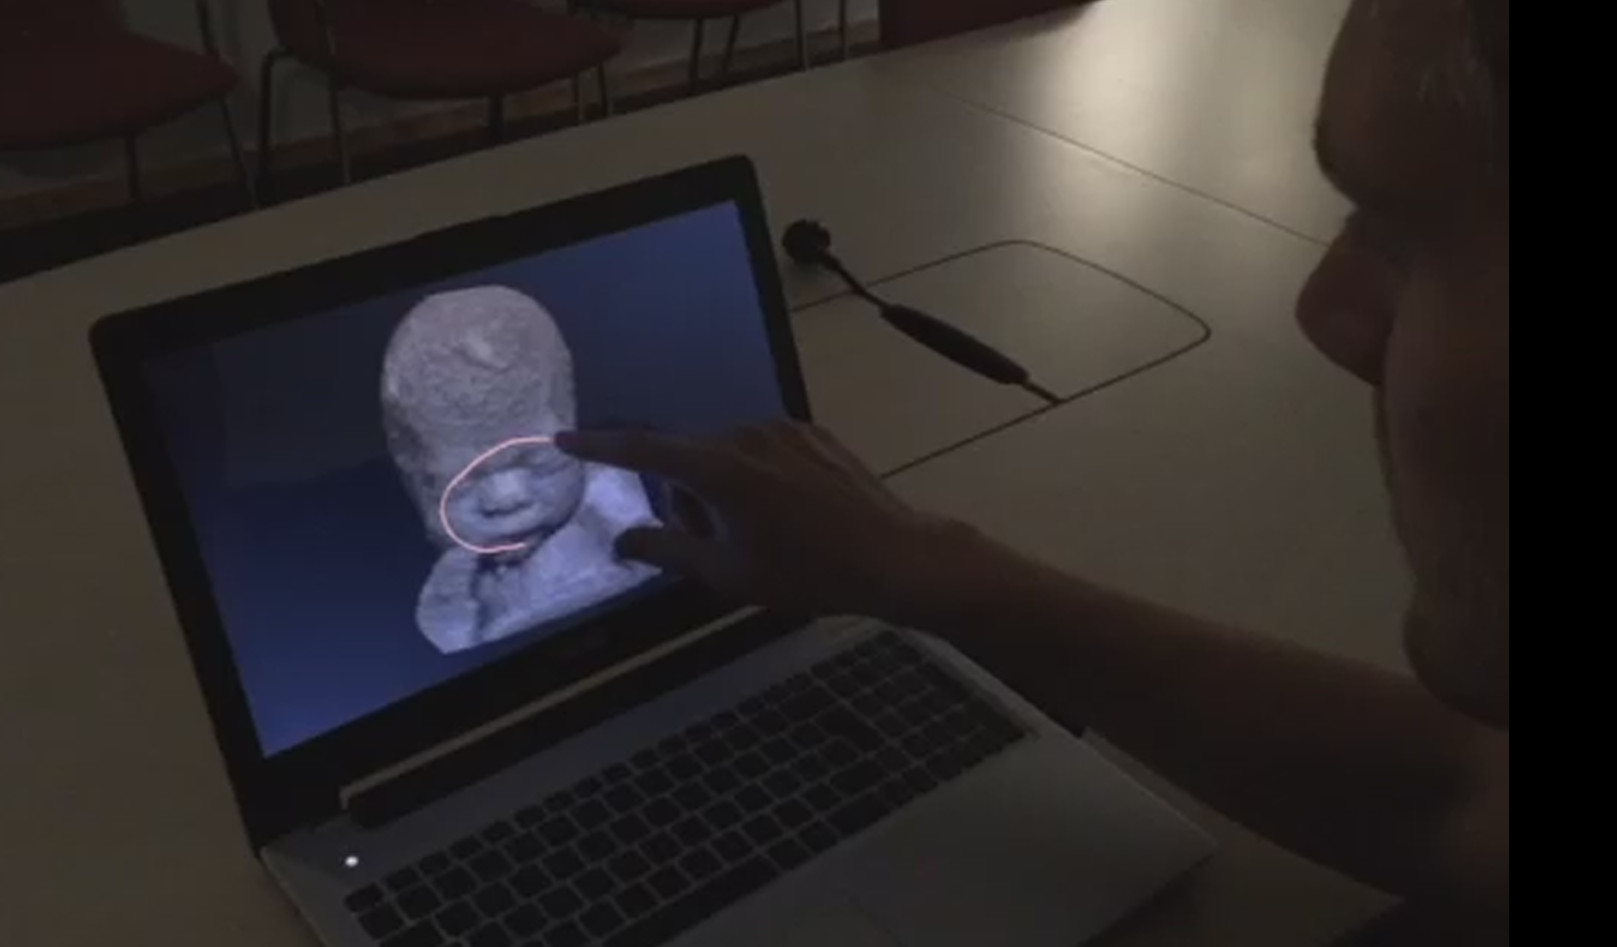
\includegraphics[width=1.0\linewidth]{images/touch_workstation}}
	\caption{Workstation: Touch screen}
	\label{img:touch_workstation}
\end{figure}

\section{(Erik) Scenario: Exhibition Area}

Both user and viewer centered.

Touch more relevant and touchless less relevant?

However, our observation has showed that touchless interaction could benefit substantially for 2D/3D objects connected to the movement, such as the hand in the penguin picture.

\begin{figure}[htb]
	\centering
	\fbox{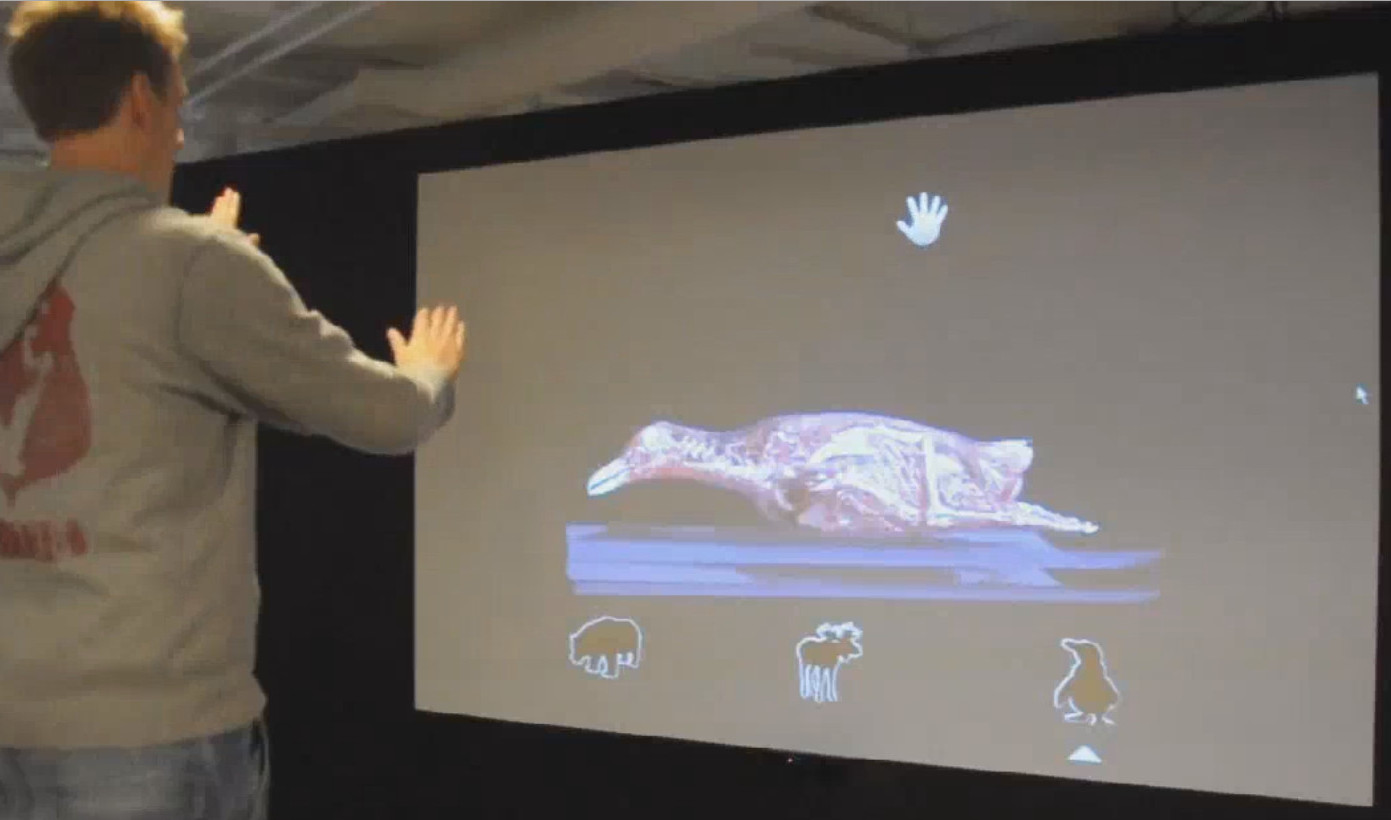
\includegraphics[width=1.0\linewidth]{images/exhib_rotate_peng}}
	\caption{Exhibition: Kinect, hand symbol supporting user and viewer guidance.}
	\label{img:exhibition_kinect}
\end{figure}

\begin{figure}[htb]
	\centering
	\fbox{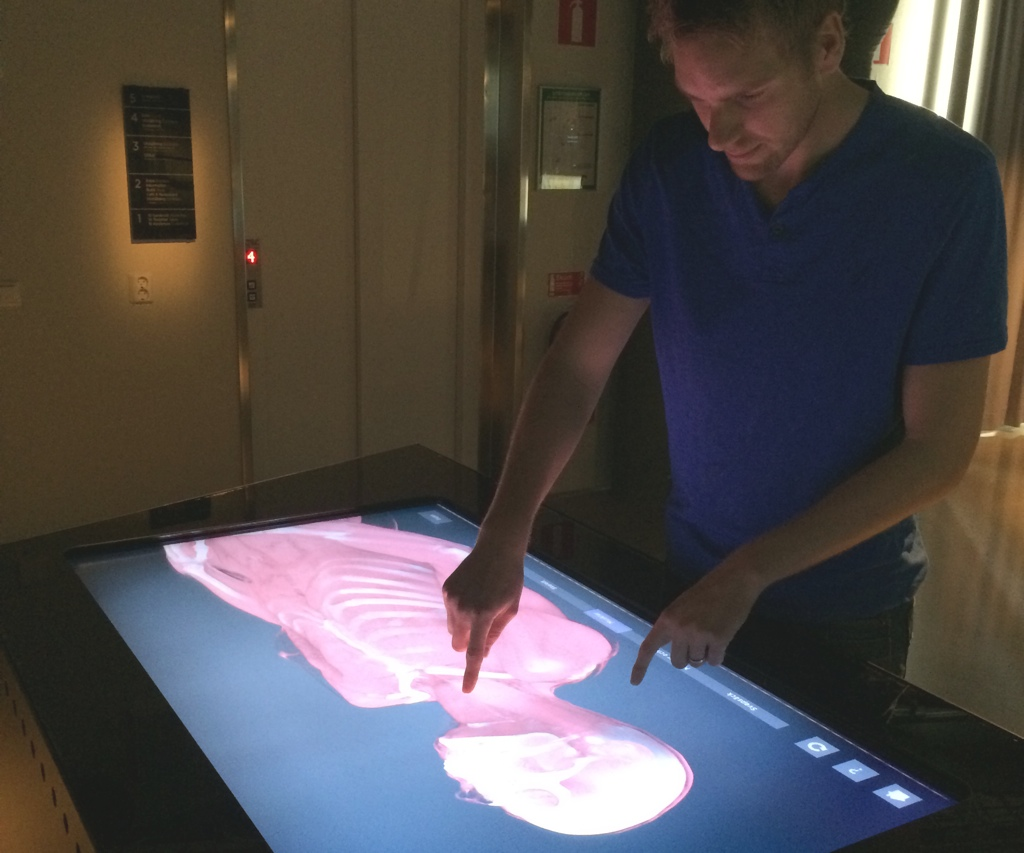
\includegraphics[width=1.0\linewidth]{images/exhib_table}}
	\caption{Exhibition: Touch Table}
	\label{img:exhibition_table}
\end{figure}

...

\section{(Alex) Scenario: Large Audience Presentation}

Viewer(Audience) centered.

Presenter is always decoupled from the screen, as the presenter can not interact with the complete presentation surface. This is often due to the lack of touch capability, but foremost the sheer size of common screens for large audience presentations can not be reached from a standing location by the user.

Dome, movement, viewers benefit to see how presenter interacts with the data.
Thus, big 3D gestures better then gesture on touch device.

User should be standing in such away that the 3D movements the user performs can be projected correctly onto the screen.

Discuss interaction option made by audience, pros and cons

\begin{figure}[htb]
	\centering
	\fbox{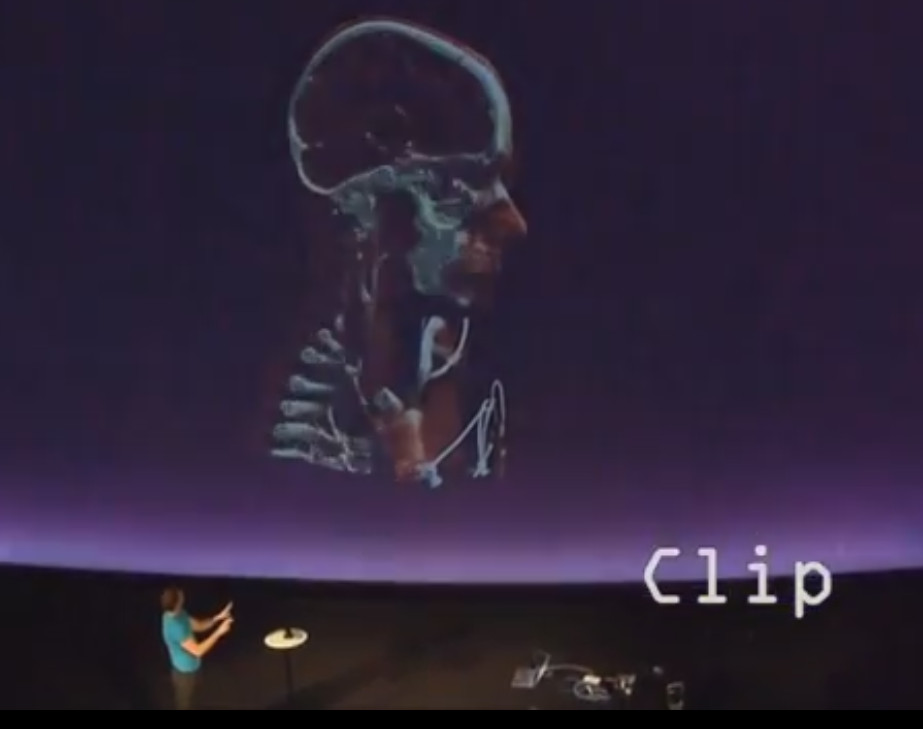
\includegraphics[width=1.0\linewidth]{images/dome_clip}}
	\caption{Dome}
	\label{img:dome_clip}
\end{figure}

\begin{figure}[htb]
	\centering
	\fbox{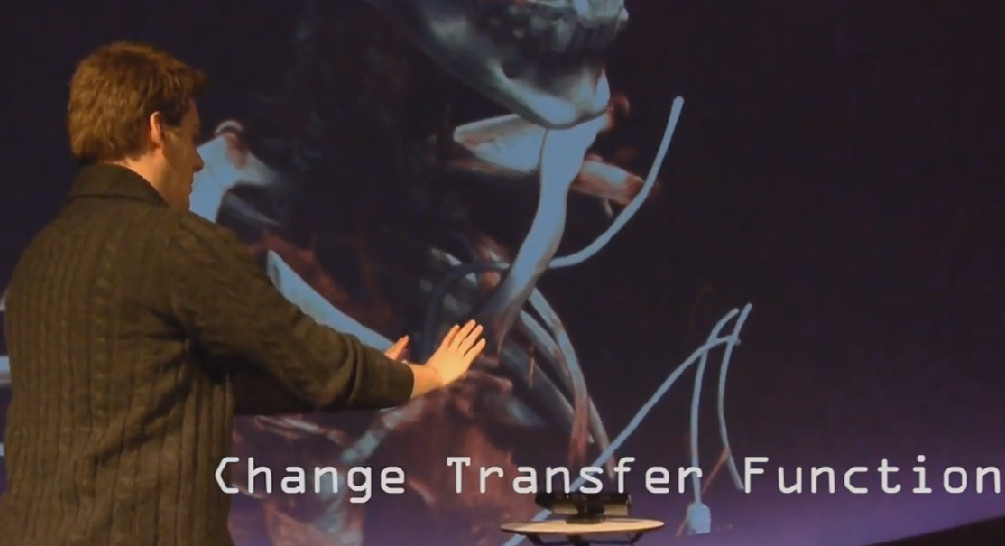
\includegraphics[width=1.0\linewidth]{images/dome_tf_change}}
	\caption{Dome Closeup}
	\label{img:dome_tf_change}
\end{figure}

\section{Conclusions}\label{sec:conclusion}

A decoupled interaction approach is always less intuitive then one which the viewing surface and interaction area is the same.

However, when a decoupled approach is necessary certain elements can be introduced in order to help the audience.

Such as projecting the hand onto the viewing surface.

\section{Future Evaluations of these scenarios}\label{sec:future}

Based on our observations we deem that an expansion of the research within viewer or audience centered interaction methods would be beneficial.

Within this subject, expert and none expert viewers have different ways of thinking and experiencing data exploration. Thus, the naturalness of the interaction could does be completely different for the different viewers.

\bibliographystyle{abbrv}
%%use following if all content of bibtex file should be shown
%\nocite{*}
\bibliography{literature}
\end{document}
